\documentclass[12pt]{upenndiss}

%bibliography
\usepackage{natbib}
\bibpunct[:]{(}{)}{,}{a}{}{,}

% phonological examples
%\usepackage{simplex}
\usepackage{amsmath}

% fonts
%\usepackage{mathspec}
%\setmainfont[Mapping=tex-text]{Linux Libertine}
%\setmathfont(Digits,Greek,Latin){Linux Libertine}
%\usepackage{microtype}
%\usepackage{coptic}


% tables and figures
\usepackage{booktabs}
\usepackage{graphicx}
\usepackage{floatrow}
\usepackage{multirow}
\usepackage{enumitem}
\newfloatcommand{capbtabbox}{table}[][\FBwidth]
\setlist{noitemsep}

% Add packages and definitions you want to use here:
\usepackage{times}
\usepackage{multirow,sectsty}
\usepackage{setspace}
\usepackage{subfigure,graphicx}
\usepackage{amsmath,amsthm,amsfonts, amssymb}
\theoremstyle{definition} \newtheorem{definition}{Definition} 
\usepackage{linguex}
% \usepackage{betababel}
\usepackage[english,greek]{betababel}
\usepackage{tikz-qtree}
\usepackage{tikz}
\usetikzlibrary{arrows,automata,chains,matrix,positioning,scopes}

\usepackage[normalem]{ulem}

\usepackage{pdfpages}

\usepackage{natbib}

\usepackage{epigraph}
\usepackage{hyperref}

 \usepackage[only, llbracket,rrbracket]{stmaryrd}
 \newcommand{\sem}[1]{\ensuremath{\{ #1 \} }}
 \newcommand{\pair}[1]{\ensuremath{\langle #1 \rangle}}
 \newcommand{\la}{\ensuremath{\lambda}}
 \newcommand{\inter}[1]{\ensuremath{\llbracket#1\rrbracket}}

\newcommand*\circled[1]{\tikz[baseline=(char.base)]{
            \node[shape=circle,draw,inner sep=2pt] (char) {#1};}}


\newcommand{\comm}[1]{}
\long\def\symbolfootnote[#1]#2{\begingroup%
\def\thefootnote{\fnsymbol{footnote}}\footnote[#1]{#2}\endgroup}

\begin{document}

\setcounter{chapter}{5}

\chapter{Chance}
\label{chance}

\setlength{\epigraphwidth}{.9\textwidth}

\epigraph{[T]o my imagination it is far more satisfactory to look at such instincts as...consequences of one general law leading to the advancement of all organic beings -- namely, multiply, vary, let the strongest live and the weakest die.\\--Charles Darwin \citeyearpar{darwin1859}}

%\\ \hspace{12pt}
%
% God does not play dice with the world.\\--Albert Einstein}


%Finally, it may not be a logical deduction, but to my imagination it is far more satisfactory to look at such instincts as the young cuckoo ejecting its foster-brothers,�ants making slaves,�the larv� of ichneumonidea feeding within the live bodies of caterpillars,�not as specially endowed or created instincts, but as small consequences of one general law leading to the advancement of all organic beings,�namely, multiply, vary, let the strongest live and the weakest die.

In our analyses of historical change we have used mean dynamics that presuppose effectively infinite populations. This assumption allows us to smooth out chance occurrences and study the expected motion of what is arguably a stochastic process. However, as we noted in the previous chapter, this does not rule out the possibility that the changes we observe are actually due to chance. Here we relax the assumption of effectively infinite populations and determine its effect on the acquisition dynamics. While the acquisition dynamics predict stability, it is only a weak kind of stability stemming from the size of the population. Either of the transitions of the formal cycle could be the result of random sampling errors in a finite rather than an infinite population.  This is particularly relevant for the second transition from \textit{\color{blue} ne...not} to \textit{\color{green} not}, which we noted cannot be explained by either use or acquisition. In this chapter we investigate the possibility that the transitions of the formal cycle are indeed due to chance.

%\textit{\color{blue} ne...not} and \textit{\color{green} not}  versus  \textit{\color{red} 

First, we briefly discuss the conceptual role of drift in the history of population genetics. Whereas early approaches to population genetics from Darwin on have emphasized selection over drift, more recent work has developed tools for addressing both theoretical possibilities. Second, we demonstrate the dynamics of drift in finite populations. We show that change can indeed come about through drift.  More importantly, we show that drift can lead to change that exhibits the qualitative trajectories so frequently observed in historical linguistics, and selection can lead to change that is decidedly not like what we observe historically. Third, we introduce a statistical method for testing whether we can reject the hypothesis of drift in favor of selection for a particular trajectory. We apply this test to both of the transitions of the formal cycle and show that while we can reject the possibility of drift in the transition from  \textit{\color{red} ne} to \textit{\color{blue} ne...not}, we cannot reject it in the transition from \textit{\color{blue} ne...not} to \textit{\color{green} not}. Finally, we discuss these results in light of the previous chapters. Given that we can reject the role of drift in the first transition, this adds support for our model of the functional cycle. Given that we cannot reject the role of drift in the second transition, we can make sense of the varying times to completion of the transition across languages.

The main contributions of this chapter are twofold. First, we offer the first application of statistical methods for distinguishing between selection and drift in linguistic time series. This has important implications not just for the formal and functional cycles, but for linguistic change as a whole. The crucial fact is that the typical trajectories observed in linguistic change may arise from selection or drift. Simply put, we cannot distinguish between these two possibilities from simple visual examination. Rather, we need a means of testing competing hypothesis about the underlying cause of the change. Second, the application of these methods offers insight into the formal cycle, and the second transition in particular given that neither use nor acquisition offer an explanation. More broadly, it also offers constraints on the nature of stable variation.


\section{Drift}

The nineteenth century saw both the discovery of the mechanics of genetic inheritance by Gregor Mendel and the formulation of the principle of natural selection by Charles Darwin. Yet, it was not until the early twentieth century that these two notions were reconciled and put on a rigorous mathematical foundation by the work of Fisher, Sewall Wright, and Haldane in what has become known as the modern \emph{evolutionary synthesis} \citep{huxley1942}. As the term suggests, these foundations offer a coherent and compelling view of observed changes in biological populations. 

The role of random drift in explaining these changes, however, was taken to be minimal in comparison to selection. The balance between selection and drift was revisited most notably by \cite{kimura1968} in his \emph{neutral theory} of evolution, which emphasized the role of drift rather than selection at the molecular level. While the proper emphasis on of each has been the subject of intense debate, more recent work in population genetics has taken the balance between these two forces as an empirical matter, developing theoretical tools for distinguishing the potential role of each.  In what follows, we adopt this approach to understanding changes in a population over time. 

In particular, our goal will be to test the role of drift in both of the transitions of the formal cycle. Our first step towards this approach is to demonstrate the need for statistical methods for distinguishing the quantitative signatures of selection versus drift in linguistic time series. We do so by simulating the dynamics of change in a finite population to demonstrate some counter-intuitive possibilities regarding drift versus selection.

% at drift can look like what we would expect of selection and selection can look what we would expect of drift, simply due to random sampling. If this is the case, then we need statistical tools for distinguishing between the two.  This is particularly important for the formal cycle if we want to know whether either of the transitions could happen simply due to random drift from one grammar to another. 


\section{Dynamics}

Here we outline the dynamics of a simple model of change in a finite population. Using simulations of the \emph{Moran model} \citep{moran1958}, we show that our intuitions about how drift and selection look are not as useful as we might think. That is, we cannot simply look at the trajectory of a change and determine intuitively if it occurred due to selection or drift. This is true despite the fact that we often observe a similar qualitative \emph{S}-shaped trajectory in the course of language change \citep{bailey1973}. 

The \emph{Moran model} describes the dynamics of selection and drift in a finite population. At each point in time one individual is chosen to reproduce and one individual is chosen to die, yielding a continuous-time Markov chain.\footnote{While the Moran model assumes continuously overlapping generations as we did in the previous chapter regarding syntactic acquisition. the \emph{Wright-Fisher model} can be taken as the discrete-time analogue where generations do not overlap and are sampled all at once. The same general point holds for the Wright-Fisher process as well though: we cannot determine the selective advantage of particular variants from the trajectory they create.} The probability that a variant is chosen to reproduce is proportional to its relative fitness. For example, consider a population composed of a particular number of two variants, $N = n_1 + n_2$. Let the selective advantage of the second variant be $s$, then  the probabilities of each being selected to reproduce are given by the following.

\begin{equation}
	p_1^{birth} = \frac{n_1}{n_1 + n_2(1+s)}
\end{equation}

\begin{equation}
	p_2^{birth} = \frac{n_2(1+s)}{n_1 + n_2(1+s)}
\end{equation}
For the case where the two variants are selectively neutral, $s=0$, the two variants are chosen directly proportional to their respective frequencies in the population. Where $s > 0$, the second variant is selected for, so the second variant is slightly more likely to be chosen. This makes sense, if one variant has a selective advantage, then we would expect it to be more likely to reproduce.

While the probability of being chosen to reproduce is proportion to the relative fitness of the two variants, the probability of being chosen to die is directly proportional to just the prevalence of the two variants in the population.

\begin{equation}
	p_1^{death} = \frac{n_1}{n_1 + n_2}
\end{equation}

\begin{equation}
	p_2^{death} = \frac{n_2}{n_1 + n_2}
\end{equation}
Given that a single individual is chosen for birth and death at each point in time, then the number of any variant either increases, decreases, or stays the same. For example, we can keep track of the number of the second variant in the population., $n_2$. This number will go up by one if an individual of the second variant is chosen to reproduce and an individual of the first variant is chosen to die. If the selections are the opposite, where an individual of the first variant is chosen to reproduce and an individual of the second variant is chosen to die,  then the number of the second variant will decrease by one in the population. If the type of both individuals selected is the same, then there will not be any change in the number of either variants. The probability of all these outcomes is determined by the probability of selection for birth and death that we listed above.

In fact, we can specify the probability of each of these changes from one point in time to the next. In particular, we can show the probability of a particular change in the number of the second variant in the population. We list the probability that $n_2$ will increase, decrease, or stay the same.

\begin{equation}
	p_{n_2,n_2+1} = p_2^{birth}p_1^{death} = \frac{n_2(1+s)}{n_1 + n_2(1+s)} \frac{n_1}{n_1 + n_2}
\end{equation}

\begin{equation}
	p_{n_2,n_2-1} = p_1^{birth}p_2^{death} = \frac{n_1}{n_1 + n_2(1+s)} \frac{n_2}{n_1 + n_2}
\end{equation}

\begin{equation}
	p_{n_2,n_2} = 1 - p_{n_2,n_2+1} - p_{n_2,n_2-1}
\end{equation}
There are two important points where the population does not change at any subsequent points in time. Namely, if $n_2 = 0$ or $n_2 = N$, then the population will not change at any point moving forward. These are referred to as the \emph{absorbing states} of the process, whereas all other states are \emph{transient}. This follows from the fact that at the absorbing states the sampling probabilities for the two variants are either one or zero. 

So, neutral selection in a finite population provides an interesting contrast to the acquisition dynamics we presented in the previous chapter. Indeed, if we loosen the assumption of an infinite population, then the acquisition dynamics makes a similarly strong prediction of no stable variation between grammars that are totally mutually incompatible. In other words, if acquisition is the only force acting on a language, then a single syntactic position will only ever be expressed by a single variant. We return to the implications of this prediction for observed stable variation below.

Now that we have specified the dynamics of the model, we can simulate trajectories of a population of size $N$ for selection coefficient $s$. Before doing so though, it is useful to consider what our expectations would be about a population evolving under neutral versus positive selection. Intuitively, we would expect selection to exhibit a clear trajectory, where the variant that is being selected against is quickly driven from the population. In contrast, we would expect neutral selection to be a more random kind of change, not necessarily tending in direction or the other. That is, we would not expect any clear trajectory favoring one variant over the other.  It is useful to dwell on these expectations a bit before considering the simulation results. We want a clear baseline to compare the results to.

When we do compare individual trajectories of the model for cases where $s=0$ versus $s >0$, we sometimes have the exact opposite results, as can be seen in Figures \ref{drift-selection} and \ref{selection-drift}. That is, in Figure \ref{drift-selection} we show the trajectory of a population under neutral selection $s=0$ that exhibits the characteristic \emph{S}-shaped curve observed in language change. Likewise, in Figure \ref{selection-drift} we show the trajectory of a population under positive selection $s=.1$ that exhibits a rather different kind of growth. The fundamental fact is that the underlying cause of a particular change cannot be read off its form, any particular \emph{S}-shaped curve may be due to drift or selection.

\begin{figure}
\begin{center}
 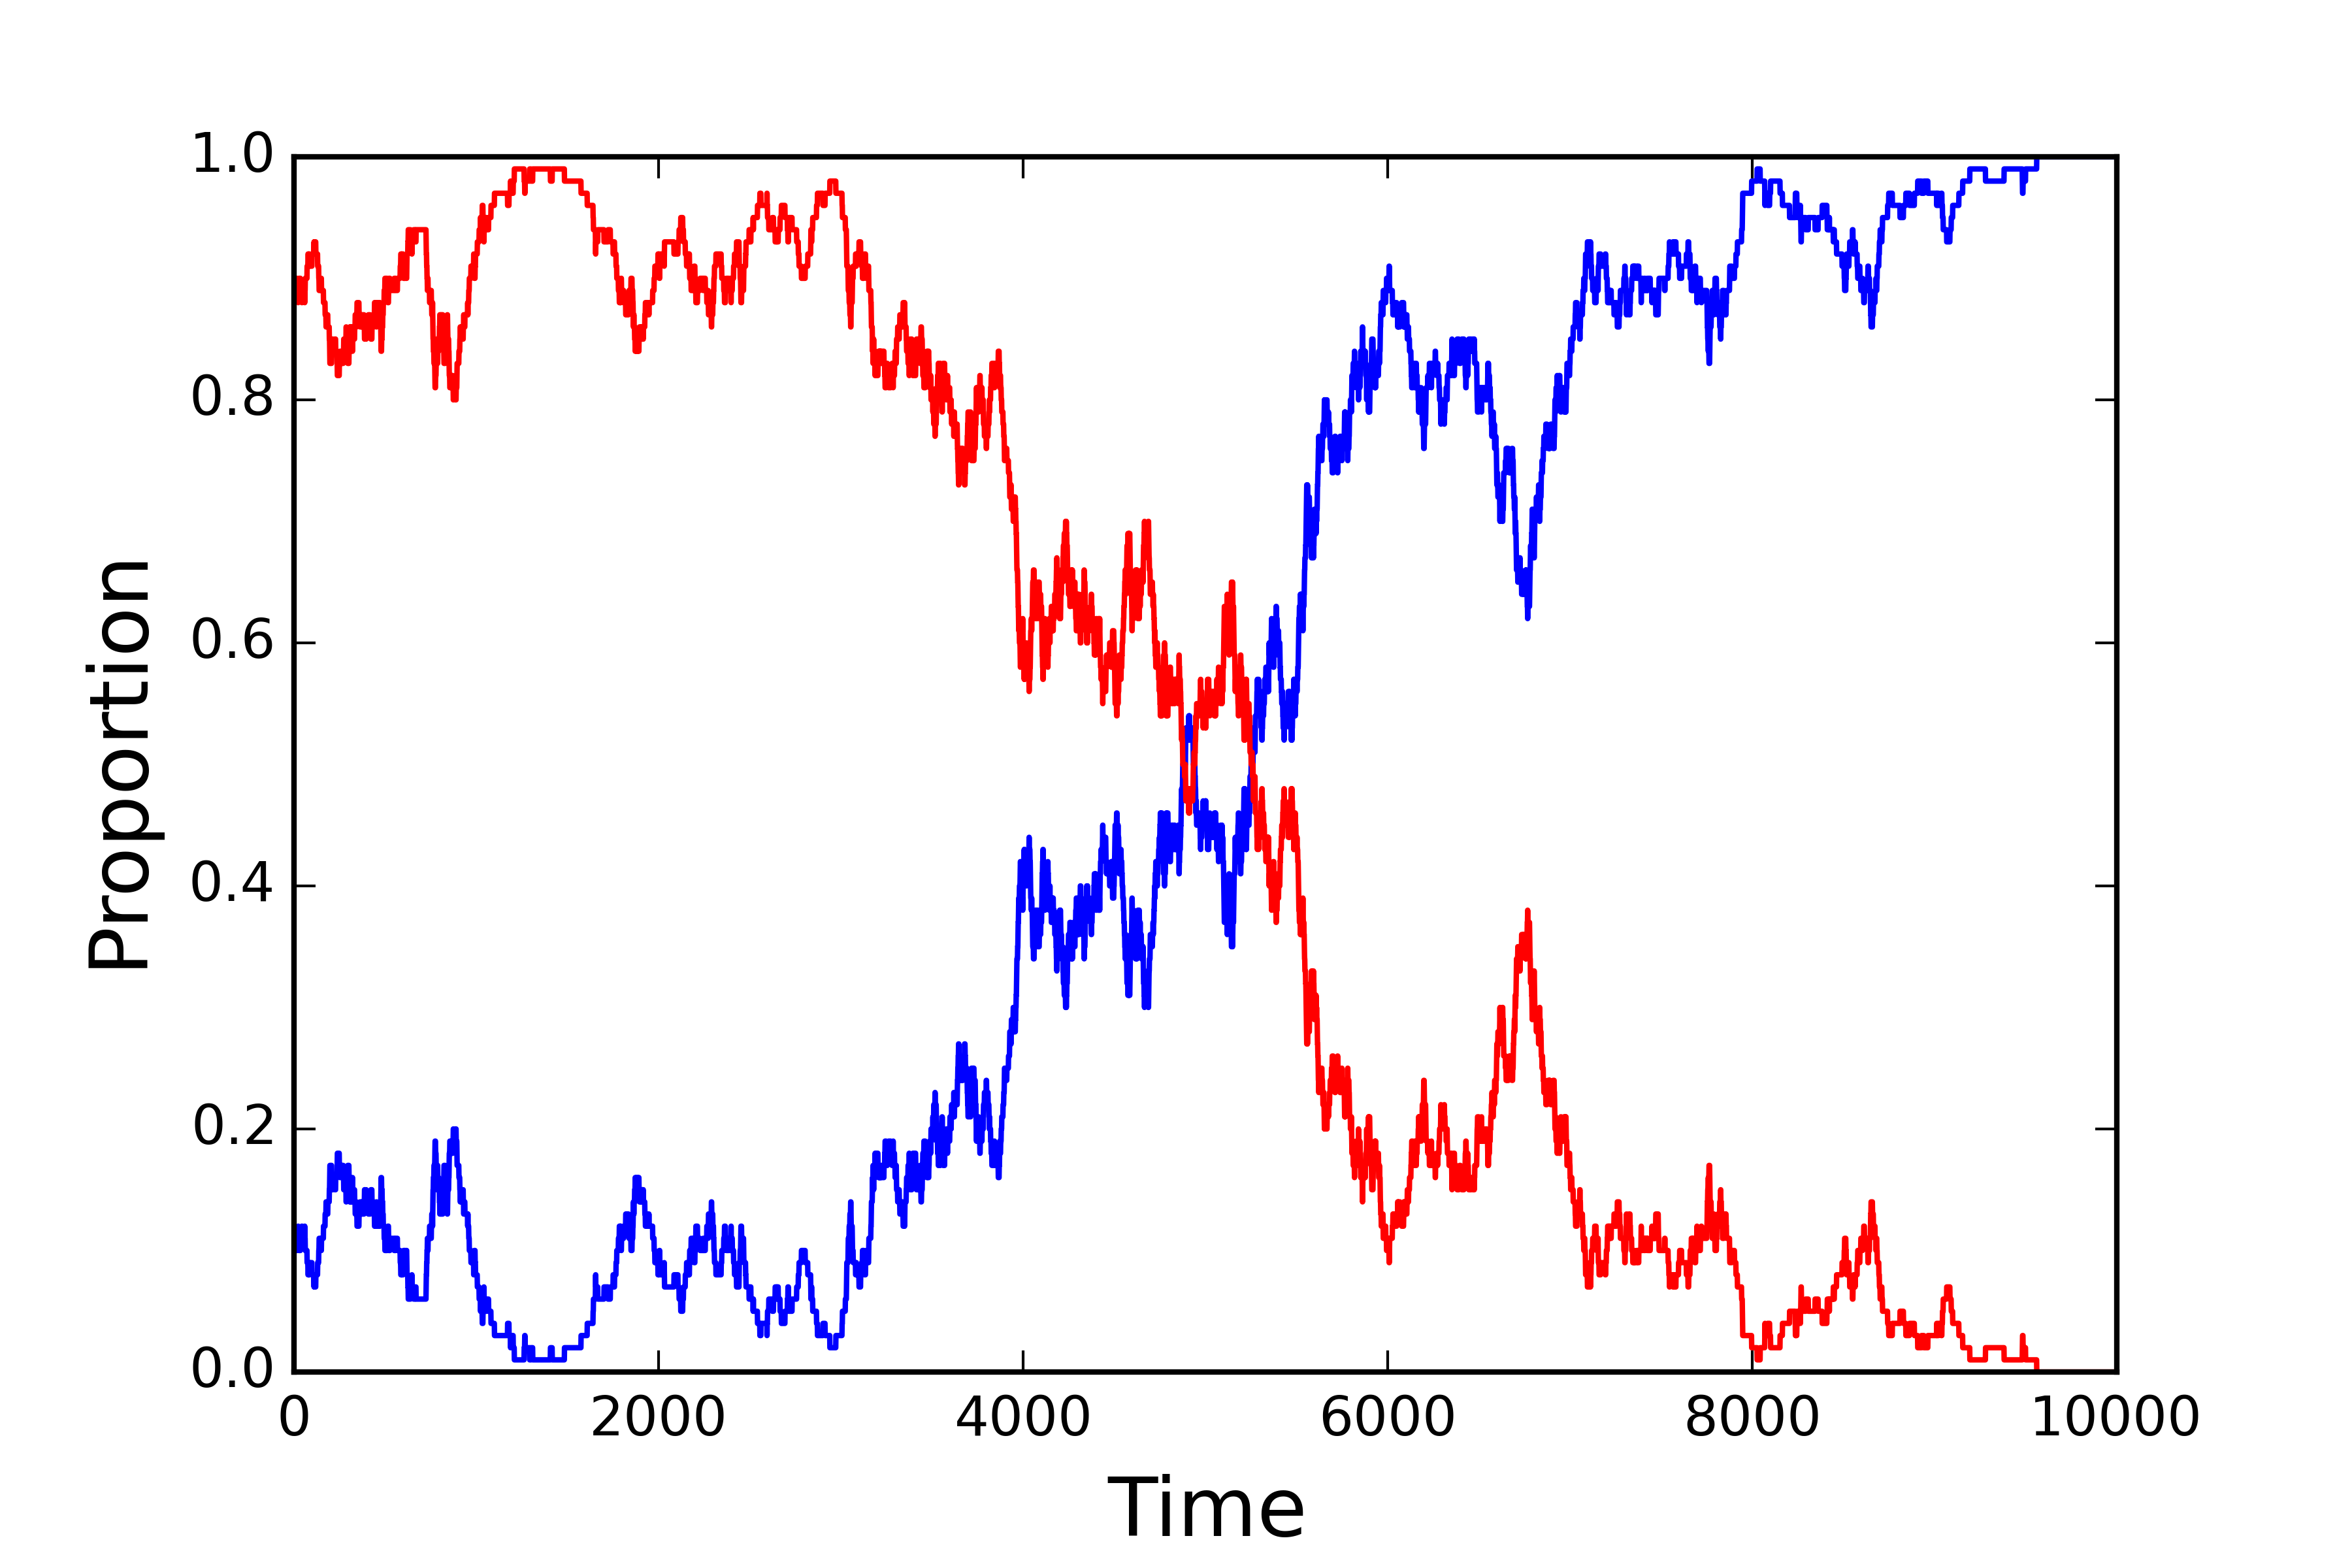
\includegraphics[width=\textwidth]{drift-selection.png}
\end{center}
	\caption{Proportion of forms over time in simulation of Moran model for $N=100$ and $s=0$}
	\label{drift-selection}
\end{figure}


\begin{figure}
\begin{center}
	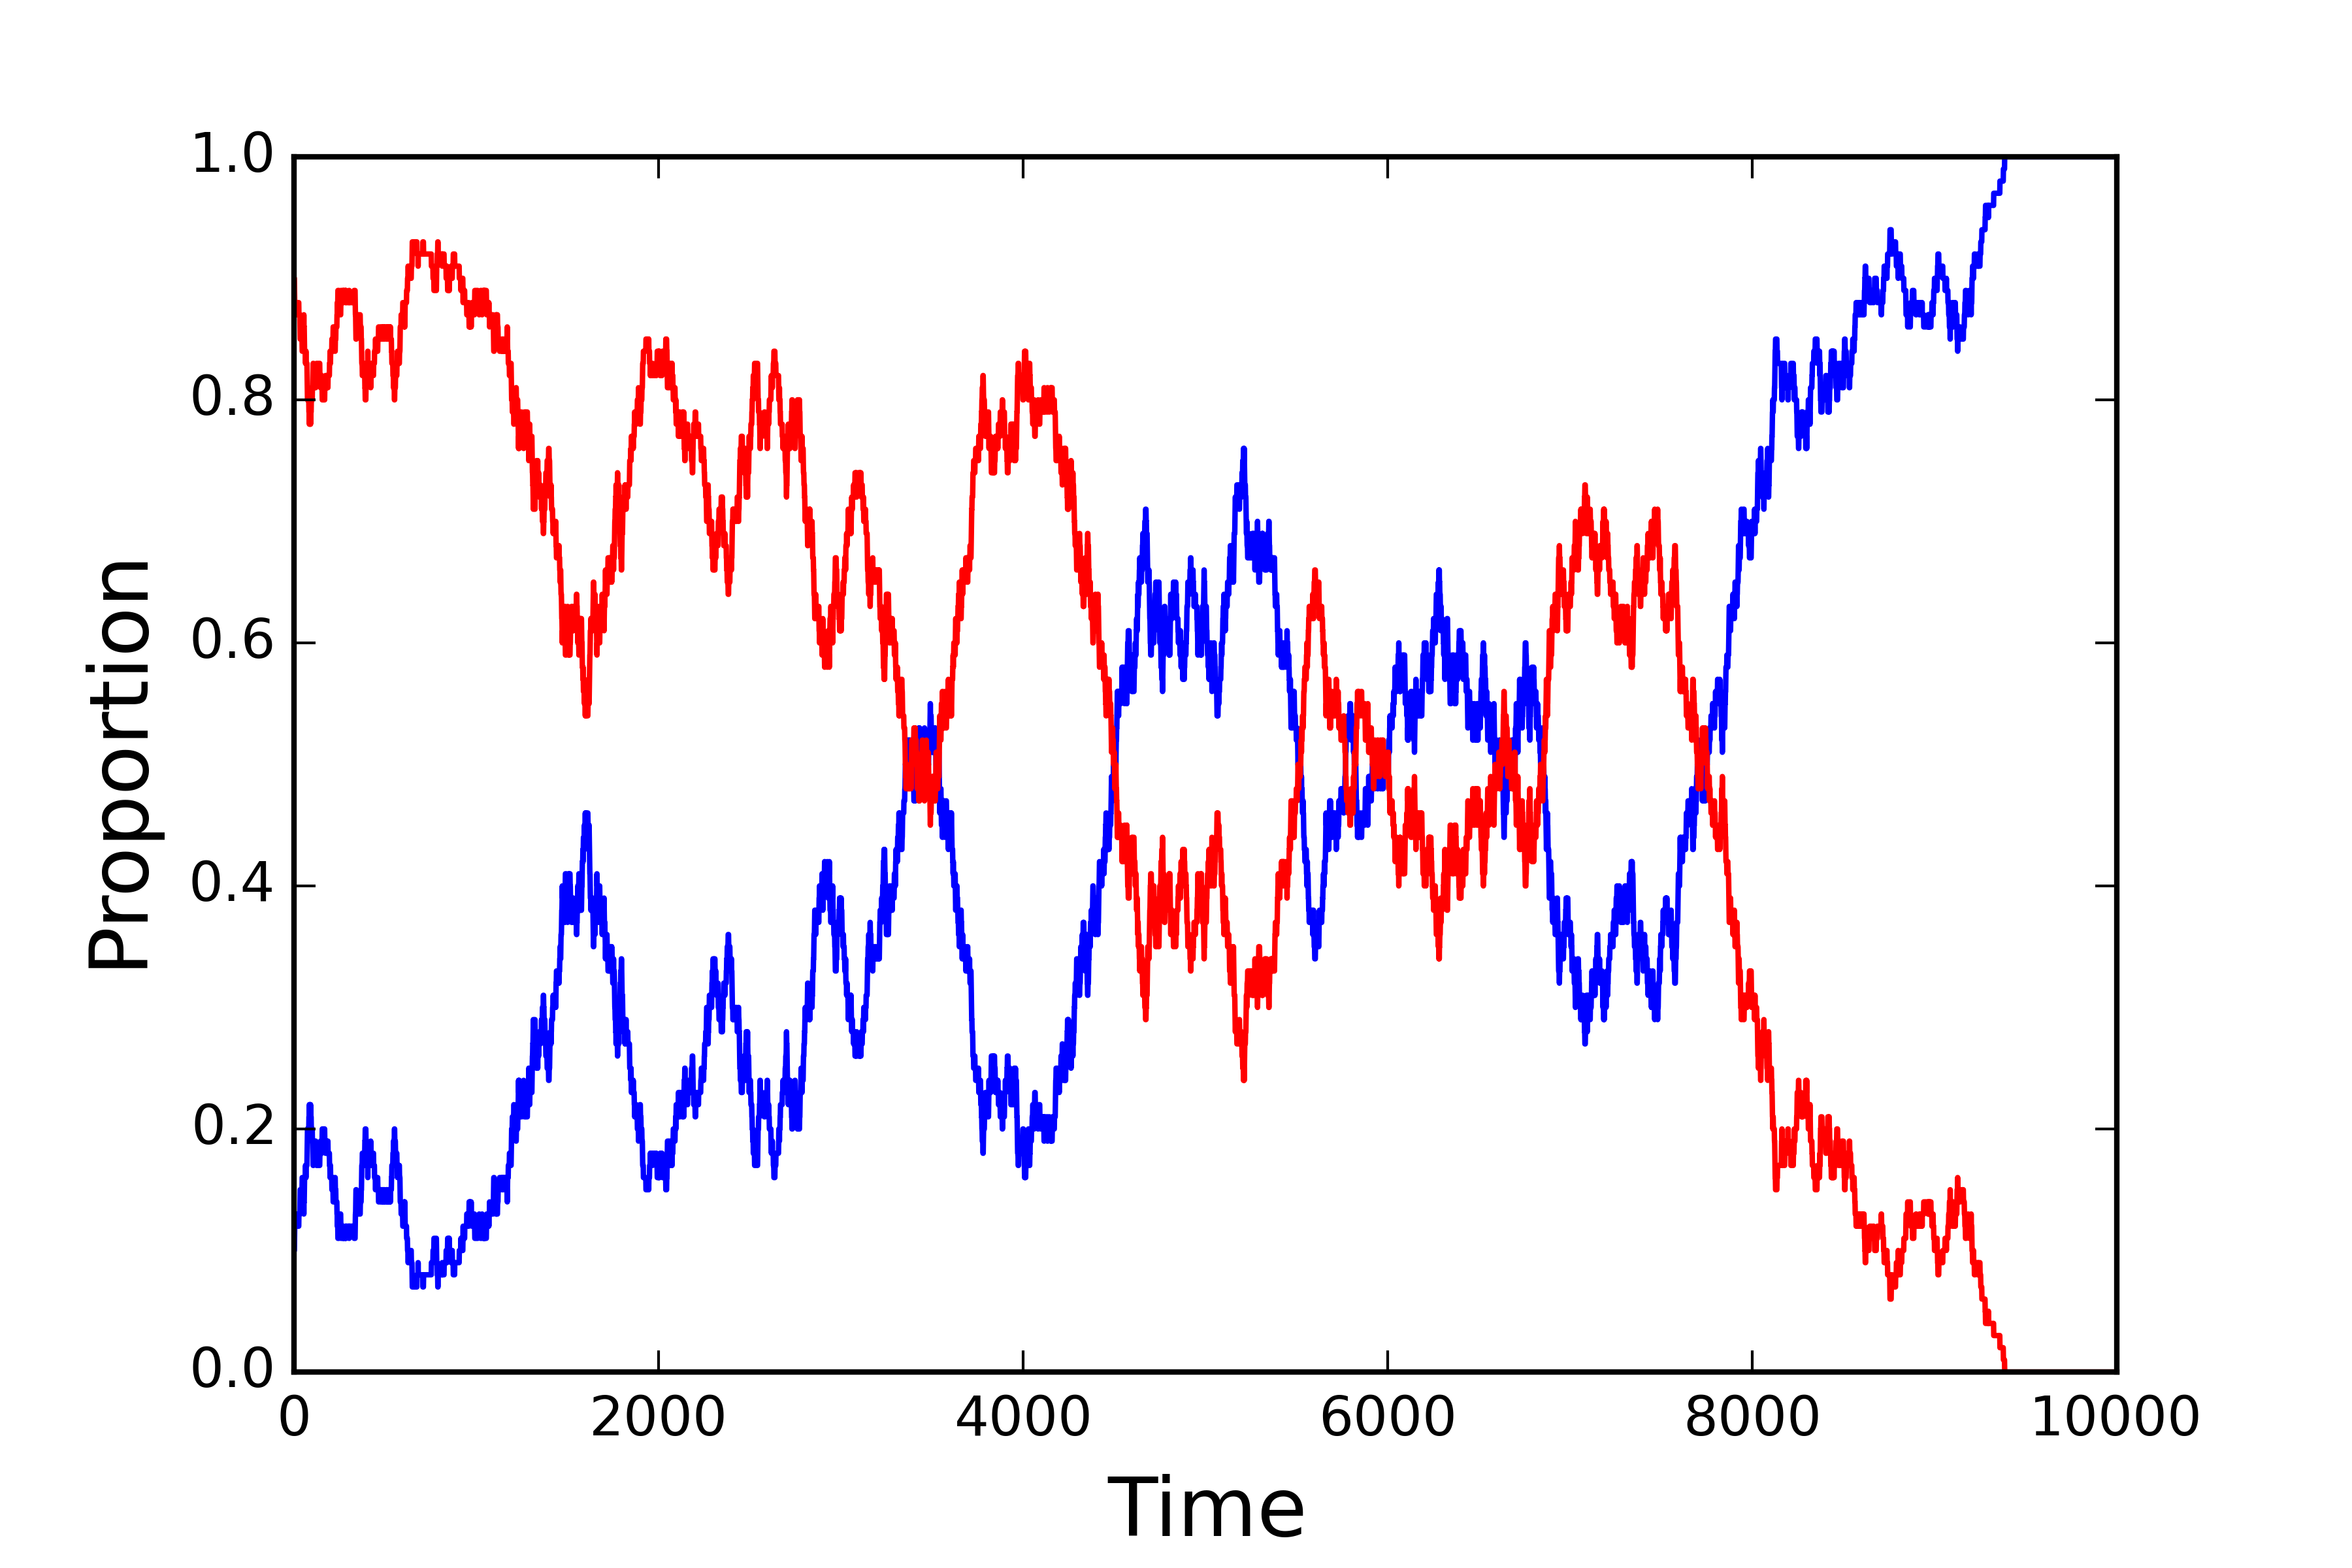
\includegraphics[width=\textwidth]{selection-drift.png}
\end{center}
	\caption{Proportion of forms over time in simulation of Moran model for $N=100$ and $s=.1$}
	\label{selection-drift}
\end{figure}

Now, one objection to this point might be that the individual trajectories presented in Figures \ref{drift-selection} and \ref{selection-drift} are atypical. More often than not, selection and drift will match our expectations. This is certainly true, these trajectories were chosen particularly to emphasize the potentially counterintuitive result of selection and drift in finite populations. So, we might be tempted to conclude that the probability that a given change is due to drift given that it is \emph{S}-shaped is actually fairly small. 

However, this objection rests on several assumptions. First, it assumes that we have some prior expectation over drift versus selection. But, we do not have sufficiently developed causal models of linguistic change that would  warrant any particular prior. In fact, in particular cases, we have very strong theoretical reasons for expecting drift, as was shown in the previous chapter regarding the transitions of the formal cycle. Second, the size of the population is not a parameter we know beforehand. That is, we can never be sure from the data itself what the probability of a particular curve should be under drift. Third, and perhaps most importantly, it is not clear what actually counts as being \emph{S}-shaped or not. While we may have intuitions about what does or does not count, these would need to be clarified.

If all of these assumptions cannot be clearly articulated and justified, then it is reasonable to assume that we simply cannot know the cause of a particular change given its shape. If this is indeed the case, then we need some means of testing different hypotheses about the underlying causes of change. For the formal cycle, we want a means of testing for whether or not each of the transitions is due to drift or selection.

\section{Modeling}

If drift and selection can yield counter-intuitive trajectories in finite populations, then we need some means of distinguishing the two in linguistic time series. In what follows, we discuss the \emph{fitness increment test} described by \cite{feder-etal2014} as a means for testing the hypotheses of drift versus selection. First, we begin by noting the motivation for the test, as well as some of details regarding its application. Second, we apply the test to the two transitions of the formal cycle.

The fundamental comparison to be made in distinguishing between drift and selection is between two models. The first model assumes that there is no selection $s=0$ and determines the population size $N$ that would best explain the data. The second model assumes that there is selection $s>0$ determines the selection coefficient and population size $N$ that would best explain the data. Given that the first model can be taken as a special case of the second, the two can be compared using a likelihood ratio test. In this case, drift is our null hypothesis and selection is our alternative hypothesis. 

However, \cite{feder-etal2014} note that doing so is not without complications. First, even using standard approximations to the Moran process \citep{kimura1955a, kimura1955b, ewens2012}, calculating the likelihoods necessary to compare the two models is computationally intensive. 
Second, even if these values were simple to obtain, the relevant test statistic is not $\chi^2$ distributed as is often assumed (cf. \citealt{wilks1938}). In fact, using the $\chi^2$ distribution systematically underestimates the false positive rate, meaning that if we assume the test-statistic is  $\chi^2$ distributed, then we will reject the null hypothesis of drift more often than we would like to when it is true.

To address these problems \cite{feder-etal2014} propose an approximation to the Moran process that consists of the combination of a deterministic logistic process and a Gaussian noise process.\footnote{See \citet[521-522]{feder-etal2014} for the mathematical details. Note that while this approximation technically only holds for the Moran process, in practice it works well for the Wright-Fisher process as well.} Under this approximation, the changes in the number of different forms over time have certain properties. Suppose we have measurements from several points in time of the two variants. Let $p_i$ be the proportion of the second variant in the population at time $t_i$. We are interested in how these proportions change over time, so will look at the differences in proportion between different points of time, $p_i - p_{i-1}$. In particular, we rescale these \emph{fitness increments} in the following manner.
\begin{equation}
	Y_i = \frac{p_i - p_{i-1}}{\sqrt{2p_{i-1}(1-p_{i-1})(t_i - t_{i-1})}}
\end{equation}

For the Gaussian approximation, under the null hypothesis of drift these scaled fitness increments are independent and approximately normally distributed around zero with a variance inversely proportional to the size of the population. In contrast, under the alternative hypothesis the increments are independent and approximately normally distributed, but with a non-zero mean and a different variance. For our purposes, we want to know whether the mean of the scaled fitness increments is greater than zero. That is, we want to know if the incoming variant has some selective advantage. This \emph{fitness increment test} can be accomplished using a one-tailed \emph{t-test}. So, under the Gaussian approximation, all we have to do to do is rescale the fitness increments and test if their mean is greater than zero.

Returning to the formal cycle, we are interested in determining whether we have sufficient evidence in favor of selection to reject the null hypothesis of drift in either of the two transitions. That is, we want to know not just whether a model with additional parameters fits the data better, but if it fits the data sufficiently better for us to reject the null hypothesis of drift. In the case of the formal cycle, we want to know whether we can reject the role of drift in the transitions from from  \textit{\color{red} ne} to \textit{\color{blue} ne...not} and from \textit{\color{blue} ne...not} to \textit{\color{green} not}.

The overall trajectory of these transitions in Middle English is shown in Figure \ref{neg-three-plot}. However, as we noted in the previous chapter, we are really interested in two independent changes at different locations in the negative phrase. In what follows, we will treat the two transitions independently. The data relevant to the first transition is shown in Figure \ref{first-plot}, where the contrast between \textit{\color{red}  ne} versus \textit{\color{blue} ne...not} and \textit{\color{green} not} indicates potential competition for what expresses the specifier of the negative phrase. The data relevant to the second transition are shown in Figure \ref{second-plot}, where the contrast between \textit{\color{green} not} versus \textit{\color{red}  ne}  and \textit{\color{blue} ne...not} indicates potential competition for what expresses the head of the negative phrase. 

\begin{figure}
\centering
     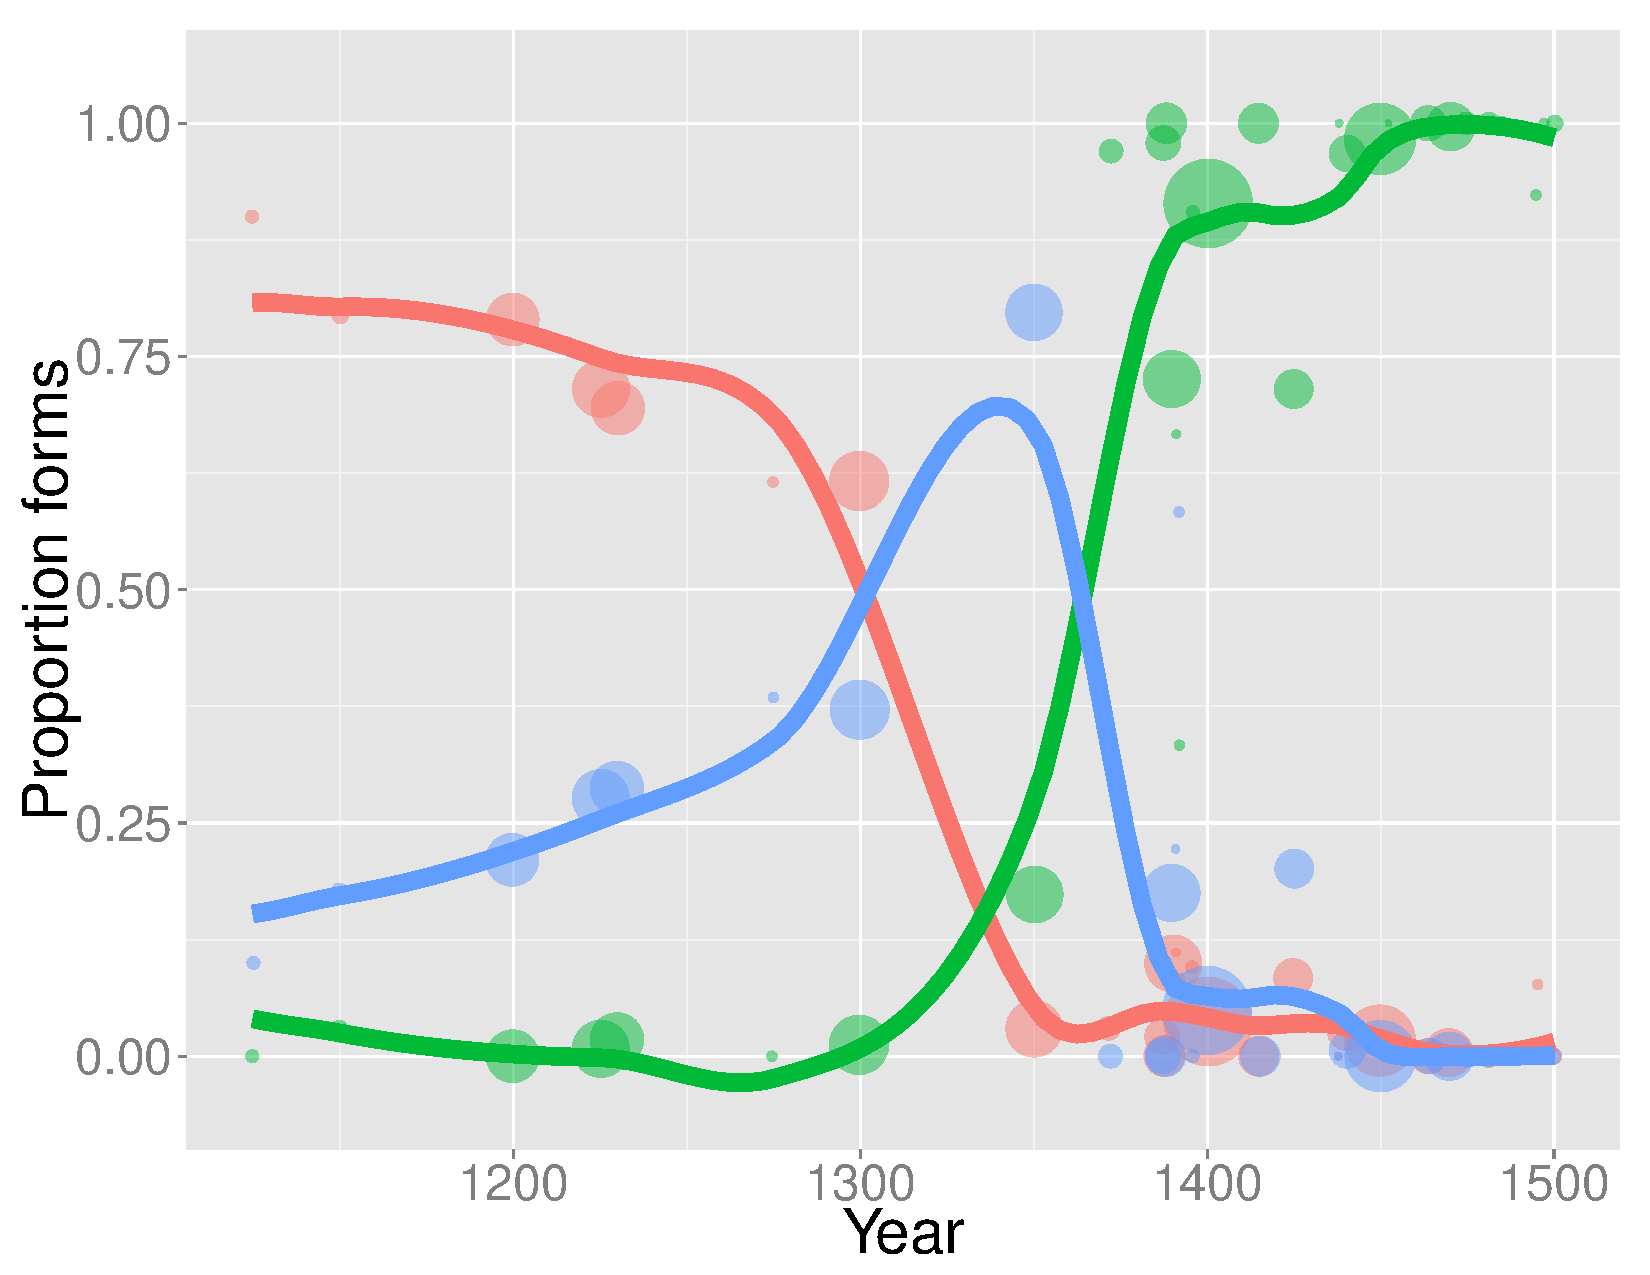
\includegraphics[width=.75\textwidth]{neg-year-lines.pdf}
\caption{Proportion of forms of negation in Negative Declaratives}
\label{neg-three-plot}
\end{figure}

\begin{figure}
\centering
     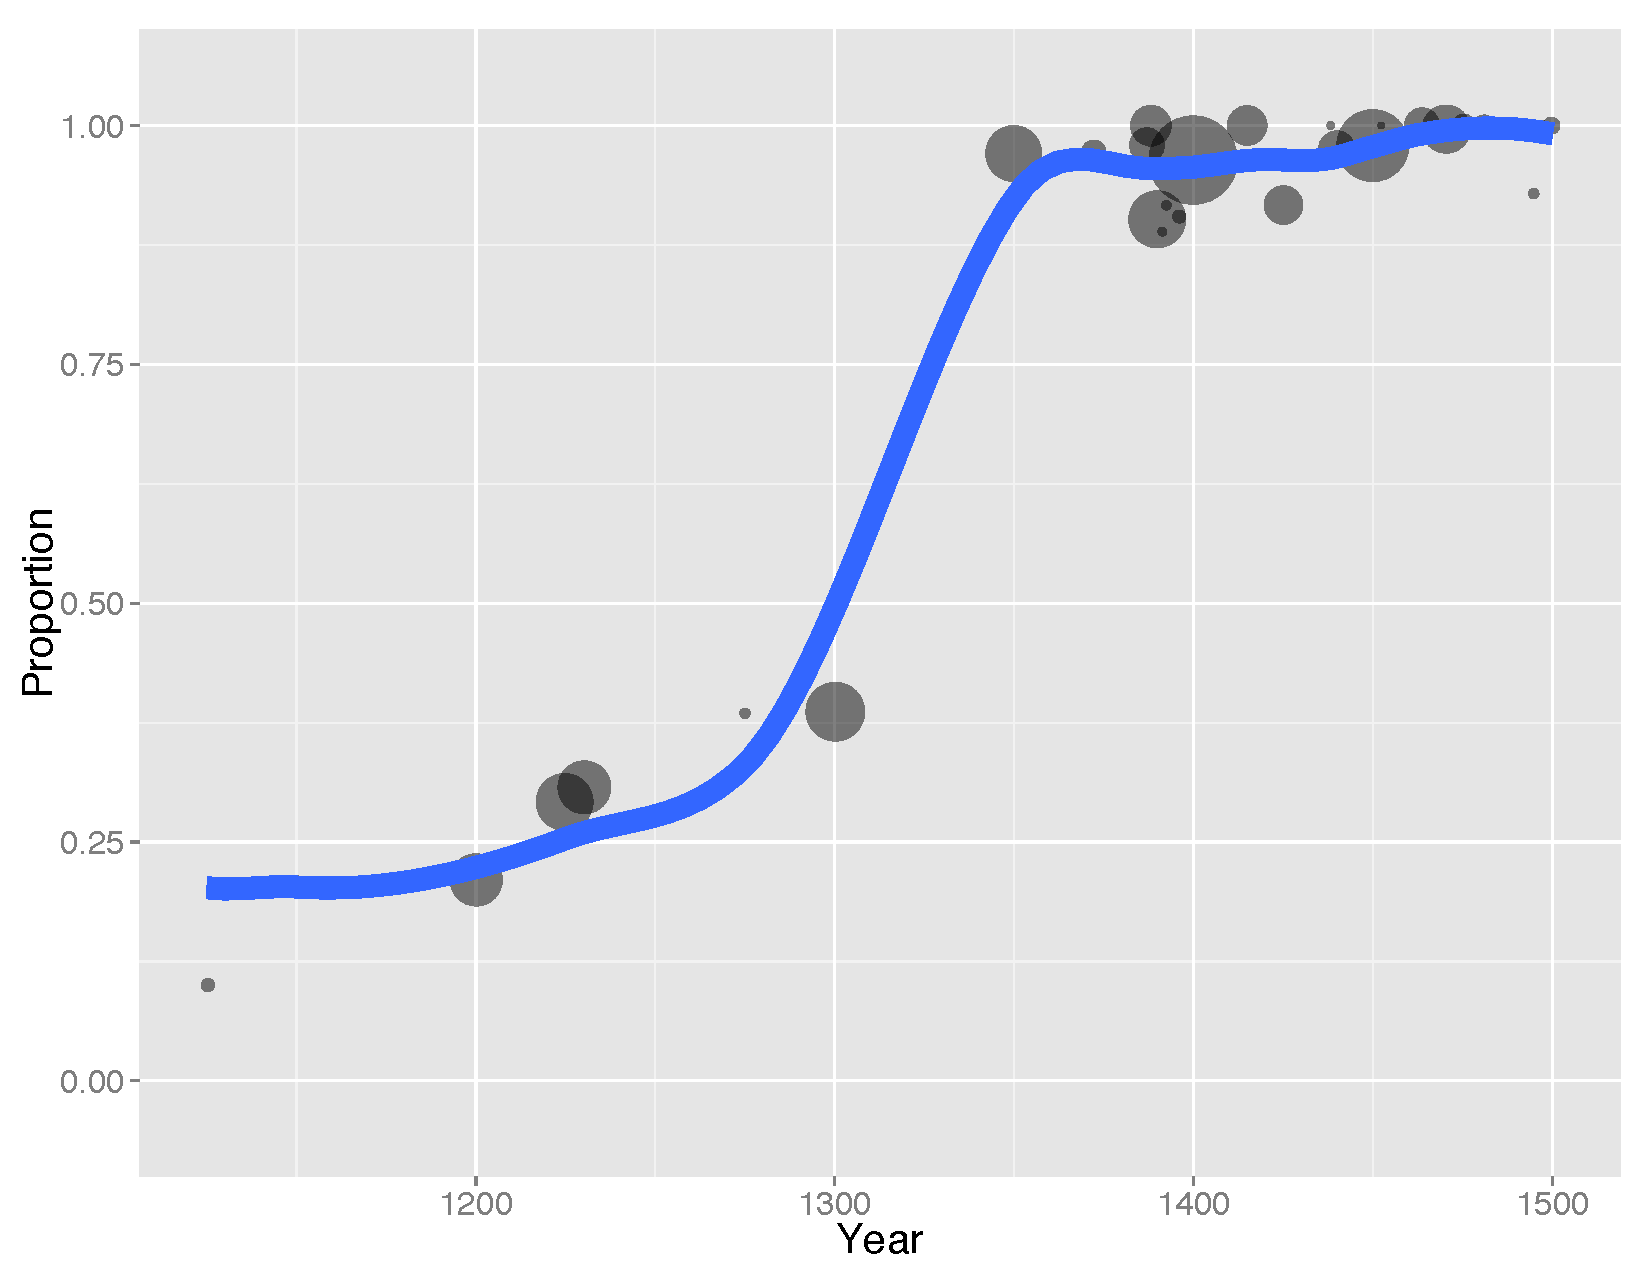
\includegraphics[width=.75\textwidth]{lump-plot1.pdf}
\caption{Proportion of \textit{\color{blue} ne...not} and \textit{\color{green} not}  versus  \textit{\color{red}  ne} over time}
\label{first-plot}
\end{figure}

\begin{figure}
\centering
     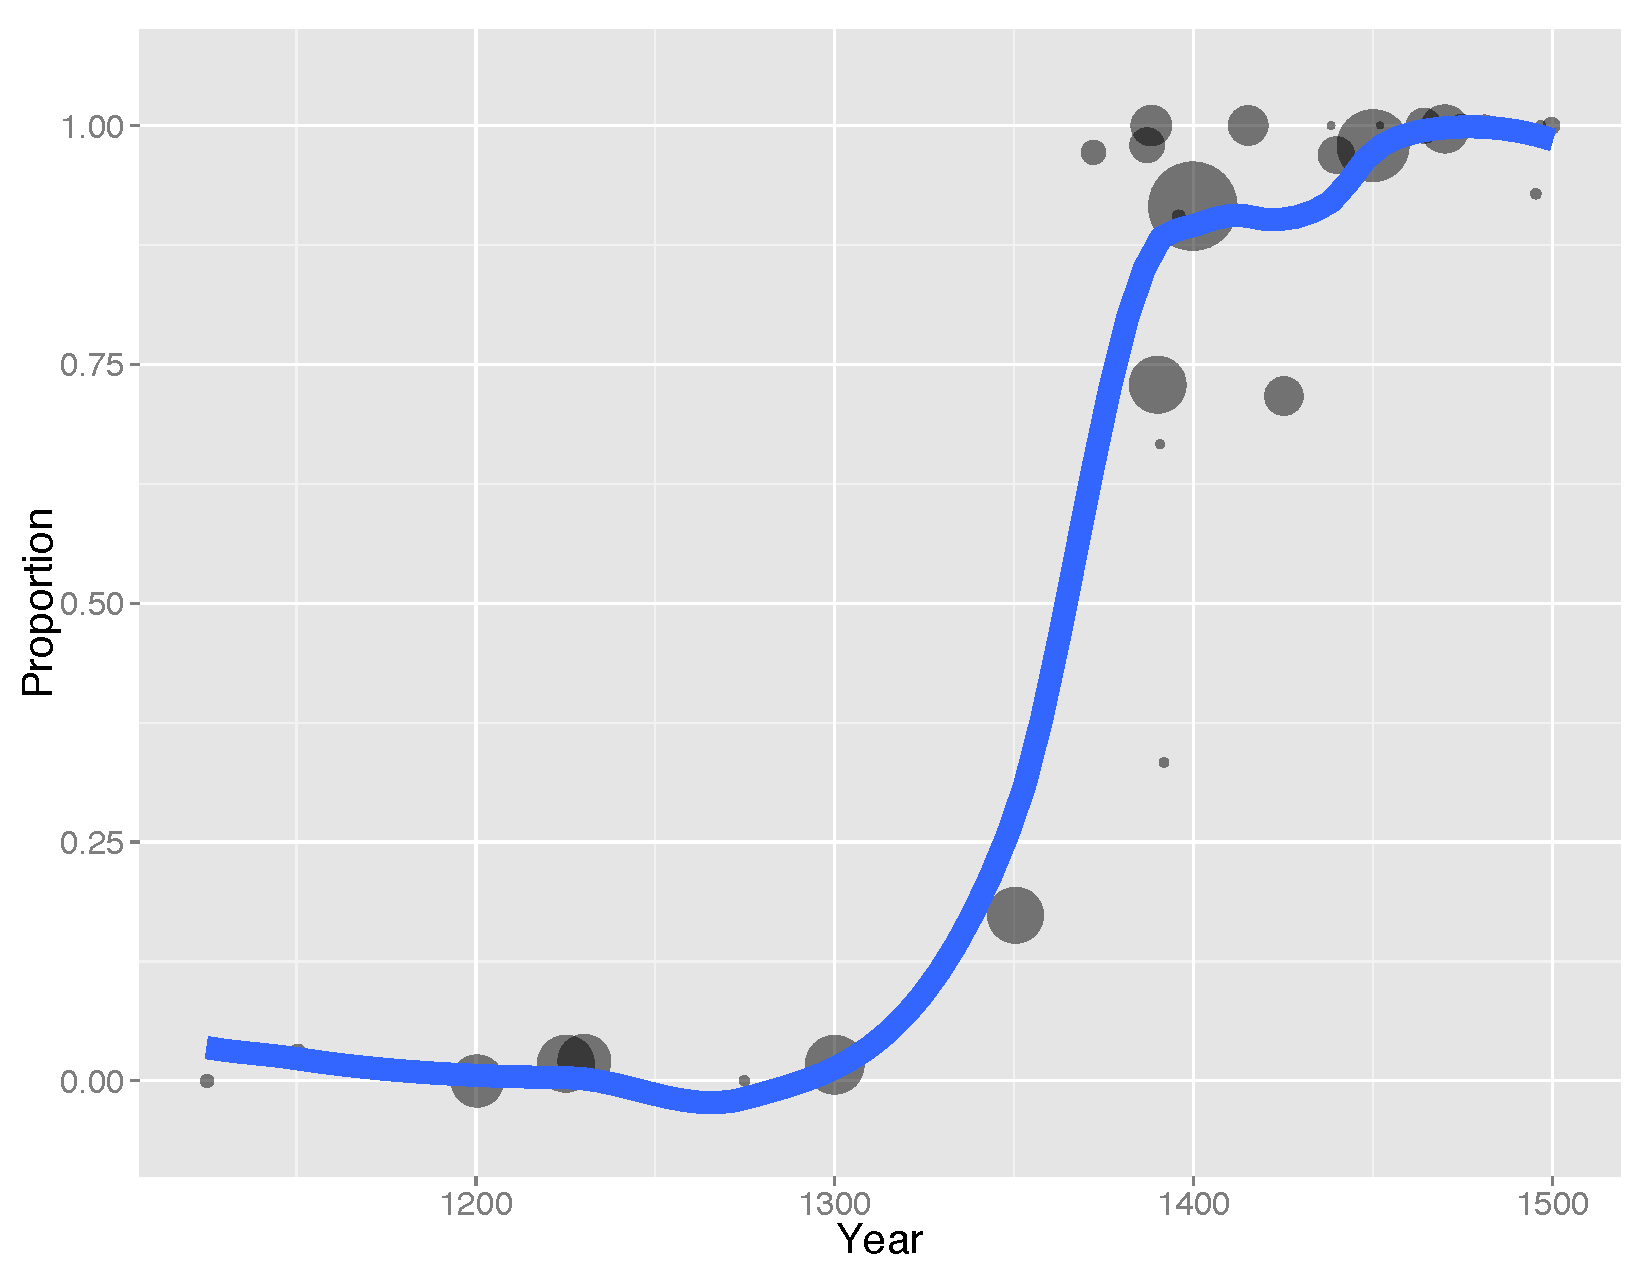
\includegraphics[width=.75\textwidth]{lump-plot2.pdf}
\caption{Proportion of \textit{\color{green} not} versus \textit{\color{red}  ne} and \textit{\color{blue} ne...not} over time}
\label{second-plot}
\end{figure}

For each of the transitions we need to decide on how to group the data together to calculate the fitness increments and perform the fitness increment test. There are two general considerations in doing so. The first consideration is that we need to make sure the assumptions of the underlying Gaussian approximation are met. In particular, the approximation cannot deal with absorption events before the last bin. If such an absorption event occurred, then all subsequent bins should be the same. So, we need to make sure there are no bins before the last one where only one variant is present. This basically serves as a limit on how finely we can bin the data.  

The second consideration is that we want the test to have as much statistical power as possible, allowing us to reject the null hypothesis when it is indeed false. In practice, the fitness increment test shows reasonable power when the increments include around a thousand data points. To guarantee that bins have approximately equal numbers of data points we bin by quantiles. This allows for the width of bins to vary, and we treat the midpoint of each bin as the time of the sample measurement.  Note that the scaling of the fitness increments takes these time differences into account as well.

So, for each transition we do three things. First, we bin the data by quantiles and perform the fitness increment test on the resulting bins. In what follows we use the finest partition of the data that give us almost one thousand data points per bin but meets the assumptions of the Gaussian approximation. Namely, there are no absorption events and the fitness increments are normally distributed. Second, we perform the fitness increment test on the rescaled fitness increments to determine if we can reject the null hypothesis of drift. Third, if we can reject the null hypothesis then we numerically estimate the mostly likely selection coefficient and population size under the alternative hypothesis of selection; if we cannot reject the null hypothesis of drift then we numerically estimate the most likely population size without selection.

For the first transition we bin the data into six bins and confirm that there are no absorption events prior to the last bin and that the rescaled fitness increments are  approximately normal according to the \emph{Shapiro-Wilk test} ($W=$, $p=0.2050$). Given that these conditions are met, we perform the fitness increment test and note that we can reject the null hypothesis of drift ($\bar{Y} = 0.0278$, $t(5)=2.6394$, $p=0.0288$). The selection coefficient and population size that best explain the data under the alternative hypothesis of selection can be numerically inferred as $\hat{s} = 0.01913$  and $\hat{N} = 15900$.\footnote{Many thanks to Mitchell Johnson for help installing and understanding the code, which can be found at \url{https://github.com/mnewberry/tsinfer}. Technically speaking, the population parameter reported here conflates another nuisance parameter regarding the time scale of the change. We leave interpreting the implications of the population parameter for future research.} While the selection coefficient from fitting the acquisition dynamics to the first transition are not directly comparable, it is interesting to note that in a finite population the selection coefficient is about five times smaller. This is a potentially important point to keep in mind when fitting deterministic mean dynamics to data.

For the second transition we bin the data into five bins and confirm that there are no absorption events prior to the last bin and that the rescaled fitness increments are approximately normal according to the \emph{Shapiro-Wilk test} ($W=$, $p=0.1300$). Given that these conditions are met, we perform the fitness increment test and note that we cannot reject the null hypothesis of drift ($\bar{Y} = 0.0624$, $t(5) = 1.7021$, $p=0.0820$). The population size under the null hypothesis of drift that best explains the data can be inferred numerically as $\hat{N}=506$. We cannot reject the null hypothesis, so it makes sense that the population would have to be fairly small to account for the rapid change in the second transition.

So, we can reject the null hypothesis of drift in the first transition, but not in the case of the second transition. This first result makes sense. given the model of the functional cycle presented in Chapter 4. That is, the first transition of the formal cycle cannot be explained by random drift in syntactic acquisition, but it can be explained as an instance of the functional cycle due to pragmatic pressures.  This second result interesting given that the second transition is the more dramatic of the changes, however, there two important things to note.

First, we have not shown that the second transition is due to drift. Rather, we have simply shown that we cannot reject the possibility. This could be due to the fact that the second transition is actually due to drift, or that we have simply failed to reject the null hypothesis even though it is not true. In this regard, we should note that the fitness increment test actually loses the power to detect selection under certain circumstances when selection is particularly strong \citep[Figure 2 and 514-515]{feder-etal2014}. However, the power of the test depends on the number of data points per bin and the length of the time series in relation to the size of the population in complicated way. Determining whether the failure to reject the null hypothesis for the second transition is due to this is something we leave for future research.\footnote{Although, these results do not change if we alter the number of bins that we divided the data into. We can never reject the null hypothesis. See Appendix D for the details.} For now though, given that we have no other alternative explanations to put forward, we lose nothing by simply noting that the second transition is consistent with random drift in syntactic acquisition.

Second, if the failure to reject the null hypothesis is indeed because the second transition is actually due to drift, then this offers an interesting explanation for the differing time courses across languages. For example, while the second transition quickly follows the first in the history of Middle English \cite{wallage2008} as well as Middle High German \cite{jager2008}. However, even in Middle Low German, where the second transition does go to completion we cannot reject drift using the data cited in \citet[109]{breitbarth2009} ($\bar{Y} = 0.02644$, $t(3) = 0.8011$, $p=0.2408$). Moreover, the second transition can take several hundred years, as is the case in the history of French \citep{martineau-mougeon2003} and Dutch \citep{burridge1993}. Indeed, some Flemish dialects still retain the embracing form \citep{vanderAuwera-neuckermans2004,zeijlstra2004}. The fact that languages differ so widely in the amount of time spent between the first and the second transition has often been taken as a puzzling. However, when the second transition is viewed as a stochastic process, the varying amount of time makes perfect sense.

Now, claiming that the second transition in all of these languages may be due to drift obscures quite a bit of linguistic detail. But, it offers both theoretical and empirical leverage. For example, if we can rule out drift quantitatively in the second transition in a particular language, then we have a compelling reason to dive into theoretical analysis of the change in question. Ultimately, such an analysis should yield explanations of the observed change similar in form to our model of the functional cycle in Chapter 4 or the acquisition dynamics we presented in Chapter 5. From the other direction, if we have compelling theoretical reasons to believe that the second transition in a language happened for a particular reason, and we can build a model that explains its trajectory, but we cannot reject the null hypothesis of drift, then this shows us some of the limitations of the quantitative methods we have applied here. 

At worst then, claiming that the second transition of the formal cycle may be due to drift is both empirically plausible and scientifically useful. Absent a better explanation, it makes sense of what has often been taken as a puzzling fact. More importantly, it clarifies what would be needed to provide a better explanation.


%\begin{table}[ht]
%\centering
%\begin{tabular}{c  l  r  l  l  l  l   r  r  l l }
%  \hline
%Bins & ML$s$ & ML$\alpha$ & LRT-P & $\overline{Y}$ & $t_{FI}$ & FIT-P & $\mu$ & $\sigma_n$ & SW-P & WX-P \\ 
%  \hline
%  4 & 0.02507 & 3270 & 0.000075 & 0.0345 & 1.3269 & 0.1579 & 1368 & 157 & 0.1691 & 0.1250 \\  
%  5 & -- & -- & -- & 0.0331 & 2.5445 & 0.0422 & 1094 & 278 & 0.1406 & 0.0625 \\  
%  6 & 0.01913 & 15900 & 0.000023 & 0.0278 & 2.6394 & 0.0288 & 912 & 197 & 0.2050 & 0.0312 \\ 
%  7 & -- & -- & -- & 0.0238 & 2.4347 & 0.0295 & 781 & 236 & 0.2185 & 0.0313 \\
%  8 & -- & -- & -- & 0.0223 & 1.4884 & 0.0936 & 684 & 129 & 0.1619 & 0.0781 \\ 
%   \hline
%\end{tabular}
%\caption{FIT on \textit{\color{red}  ne} versus \textit{\color{blue} ne...not} and \textit{\color{green} not} }
%\label{lump-table1}
%\end{table}

%\begin{table}[ht]
%\centering
%\begin{tabular}{c  l  r  l  l  l  l   r  r  l l }
%  \hline
%Bins & ML$s$ & ML$\alpha$ & LRT-P & $\overline{Y}$ & $t_{FI}$ & FIT-P & $\mu$ & $\sigma_n$ & SW-P & WX-P \\
%  \hline
%  4 & 0.05791 & 15660 & 0.000045 & 0.1316 & 1.3857 & 0.1501 & 1368 & 157 & 0.1135 & 0.1250 \\
%  5 & 0.11907 & 24 & 0.000068 & 0.0825 & 1.9787 & 0.0711 & 1094 & 278 & 0.1300 & 0.0625 \\ 
%  6 & -- & -- & --  & 0.0624 & 1.7021 & 0.0820 & 912 & 197 & 0.0052 & 0.0312 \\
%  7 & -- & -- & -- & 0.0520 & 1.5250 & 0.0939 & 781 & 236 & 0.0421 & 0.0781 \\ 
%  8 & -- & -- & --  & 0.0649 & 1.8516 & 0.0568 & 684 & 129 & 0.0157 & 0.0781 \\    \hline
%\end{tabular}
%\caption{FIT on \textit{\color{red}  ne} and \textit{\color{blue} ne...not} versus  \textit{\color{green} not} }
%\label{lump-table2}
%\end{table}


%Completion of transition from Stage II to Stage III: variable:
%HighGerman: by1300 (Dal1966:164;Lockwood1968:207f.;J�ger2006:211) English: around 1350-1420 (Wallage 2005:195) Dutch : 1600 (Burridge 1993:190f)
%BUT:
%Flemish dialects/tussentaal retain preverbal marker to this day: see van der Auwera and Neukermans 2004, Zeijlstra 2004, Van der Auwera and de Vogelaer (to appear ) for Flemish dialects in General and Haegeman 1995, 1998, 2001, 2002, 2003; Haegeman &


\section*{Summary}

In this chapter we applied statistical methods developed in population genetics to test the hypothesis of selection and drift in both transitions of the formal cycle in Middle English. We found that we could reject the null hypothesis of drift in the first but not the second transition. The result for the first transition makes sense. In fact, given the explanation of the formal cycle we offered in Chapter 4, we would be surprised if we could not reject drift in the first transition of the formal cycle. The result for the second transition also makes sense. The model we presented in Chapter 4 does not offer an explanation of the second transition. Moreover, given the syntactic structures posited to underly the formal cycle, the acquisition dynamics presented in Chapter 5 do not offer an explanation either. If neither acquisition nor use can explain the transition, then it might just be due to random drift.

Beyond the formal cycle, these results have important implications for stable linguistic variation in general.  The acquisition dynamics allow for stable variation only when grammars are perfectly mutually incompatible. That is, when $s=0$, the two grammars are perfectly balance and will not change over time. However, if we relax the assumption of an effectively infinite population that underlies this mean dynamics, we know that one or the other variant will win it. This follows from the fact that the absorbing states of the stochastic process occur where only one or the other variant is used. So, if acquisition is the only force acting on forms over time, then we will not observe linguistic variation at  a particular level. Namely, there can never be variation between how a particular syntactic location is expressed.

The fact that we do observe stable variation suggests that there are other forces acting over the distribution of forms in the linguistic environment. Indeed, in some cases stable variation has been observed over centuries, as is the case for the apical and velar variants of (ING) \citep{Labov:1994}: \emph{hunting} versus \emph{huntin'}. If not for some countervailing force, this variation should have arguably been extinguished, if these variants differ only in how they express some progressive aspectual head in the sense of \emph{distributed morphology} \citep{embick2007}. 

Broadly speaking, it would seem that the most likely candidate for a countervailing force to the monomorphic effect of syntactic acquisition is meaning, which we take to include semantic, pragmatic, and sociostylistic information. That is, the stability of (ING) arguably stems from the fact that it signals style: \emph{hunting} is formal whereas \emph{huntin'} is not. So, while two variants may compete with each other to express the same syntactic position, they might stably coexist if they find complementary informational niches.  This is exactly what we see with the specialization of the two (ING) variants to particular styles. As a slogan then, we might say: no stable variation without information. Note that this does not mean that stable informational variation is inherently stable. However, it would seem that it is more likely that two meanings might specialize rather than pool together. Of course, this is an empirical matter. One potential line of research to investigate such developments would be to employ word-embeddings to construct measures of similarity between the meanings of different variants over time. 



% Bibliography
\bibliographystyle{mcbride}
\bibliography{ahern}

\end{document}
